%% Submissions for peer-review must enable line-numbering
%% using the lineno option in the \documentclass command.
%%
%% Preprints and camera-ready submissions do not need
%% line numbers, and should have this option removed.
%%
%% Please note that the line numbering option requires
%% version 1.1 or newer of the wlpeerj.cls file, and
%% the corresponding author info requires v1.2

\documentclass[fleqn,10pt,lineno]{wlpeerj} % for journal submissions

% ZNK -- Adding headers for pandoc

\setlength{\emergencystretch}{3em}
\providecommand{\tightlist}{
\setlength{\itemsep}{0pt}\setlength{\parskip}{0pt}}
\usepackage{lipsum}
\usepackage[unicode=true]{hyperref}
\usepackage{longtable}


% Pandoc syntax highlighting
% See https://github.com/rstudio/rticles/issues/182


% Pandoc Header
\usepackage{lipsum}

\title{Template for preparing your research report submission to PeerJ using RMarkdown}

\author[1]{Charles T.Gray}

\author[2]{Ross W. Gayler}

\corrauthor[2]{Ross W. Gayler}{\href{mailto:ross@rossgayler.com}{\nolinkurl{ross@rossgayler.com}}}
\author[3]{Stefan Reimann}


\affil[1]{Charles' institution address, Australia}
\affil[2]{www.rossgayler.com}
\affil[3]{Stefan's institution address, Switzerland}


%
% \author[1]{First Author}
% \author[2]{Second Author}
% \affil[1]{Address of first author}
% \affil[2]{Address of second author}
% \corrauthor[1]{First Author}{f.author@email.com}

% 

\begin{abstract}
The abstract of the article. It can also be on \emph{multiple} lines.
% Dummy abstract text. Dummy abstract text. Dummy abstract text. Dummy abstract text. Dummy abstract text. Dummy abstract text. Dummy abstract text. Dummy abstract text. Dummy abstract text. Dummy abstract text. Dummy abstract text.
\end{abstract}

\begin{document}

\flushbottom
\maketitle
\thispagestyle{empty}

\hypertarget{introduction}{%
\section*{Introduction}\label{introduction}}
\addcontentsline{toc}{section}{Introduction}

Your introduction goes here! Some examples of commonly used commands and features are listed below, to help you get started.

If you have a question, please use the help menu in the top right of the screen to get in touch. When your article or pre-print is complete, use the ``Submit to PeerJ'' button in the topbar to send your files to PeerJ.

TESTING - Trying reverse symlink to output paper.

\hypertarget{about-peerj}{%
\subsection*{About PeerJ}\label{about-peerj}}
\addcontentsline{toc}{subsection}{About PeerJ}

PeerJ is an award-winning open access publisher covering the biological and medical sciences. PeerJ provides authors with three publication venues: \emph{PeerJ} and \emph{PeerJ Computer Science} (peer-reviewed academic journals) and \emph{PeerJ PrePrints} (a `pre-print server'). See \url{https://peerj.com/about/publications/} for more information.

The PeerJ model allows an author to publish articles in their peer-reviewed journal via the purchase of a lifetime Publication Plan. Prices start from just \$99 (a one-off payment) which entitles an author to the lifetime ability to publish 1 article per year for free. Publication in PeerJ PrePrints is entirely free.

\hypertarget{some-examples}{%
\section*{\texorpdfstring{Some \LaTeX{} Examples}{Some  Examples}}\label{some-examples}}
\addcontentsline{toc}{section}{Some \LaTeX{} Examples}

Use section and subsection commands to organize your document. \LaTeX{} handles all the formatting and numbering automatically. Use ref and label commands for cross-references.

\hypertarget{figures-and-tables}{%
\subsection*{Figures and Tables}\label{figures-and-tables}}
\addcontentsline{toc}{subsection}{Figures and Tables}

Use the table and tabular commands for basic tables --- see Table \ref{tab:widgets}, for example. You can upload a figure (JPEG, PNG or PDF) using the project menu. To include it in your document, use the includegraphics command as in the code for Figure \ref{fig:view} below.

Standard \LaTeX references will work as well (e.g.~Fig. \ref{fig:view}).

\begin{figure}

\includegraphics[width=1\linewidth]{view} \caption{An example image.}\label{fig:view}
\end{figure}

\begin{longtable}[]{@{}lr@{}}
\caption{\label{tab:widgets} An Example Table.}\tabularnewline
\toprule
Item & Quantity\tabularnewline
\midrule
\endfirsthead
\toprule
Item & Quantity\tabularnewline
\midrule
\endhead
Widgets & 42\tabularnewline
Gadgets & 13\tabularnewline
\bottomrule
\end{longtable}

\hypertarget{citations}{%
\subsection*{Citations}\label{citations}}
\addcontentsline{toc}{subsection}{Citations}

LaTeX formats citations and references automatically using the bibliography records in your .bib file, which you can edit via the project menu. Use the cite command for an inline citation, like Figueredo and Wolf (2009), and the citep command for a citation in parentheses (Figueredo and Wolf 2009).

\hypertarget{mathematics}{%
\subsection*{Mathematics}\label{mathematics}}
\addcontentsline{toc}{subsection}{Mathematics}

\LaTeX{} is great at typesetting mathematics. Let \(X_1, X_2, \ldots, X_n\) be a sequence of independent and identically distributed random variables with \(\text{E}[X_i] = \mu\) and \(\text{Var}[X_i] = \sigma^2 < \infty\), and let
\[S_n = \frac{X_1 + X_2 + \cdots + X_n}{n}
      = \frac{1}{n}\sum_{i}^{n} X_i\]
denote their mean. Then as \(n\) approaches infinity, the random variables \(\sqrt{n}(S_n - \mu)\) converge in distribution to a normal \(\mathcal{N}(0, \sigma^2)\).

\hypertarget{lists}{%
\subsection*{Lists}\label{lists}}
\addcontentsline{toc}{subsection}{Lists}

You can make lists with automatic numbering \dots

\begin{enumerate}
\def\labelenumi{\arabic{enumi}.}
\tightlist
\item
  Like this,
\item
  and like this.
\end{enumerate}

or bullet points\ldots{}

\begin{itemize}
\tightlist
\item
  Like this,
\item
  and like this.
\end{itemize}

or with descriptions\ldots{}

\begin{itemize}
\tightlist
\item
  \textbf{Word} Definition
\item
  \textbf{Concept} Explanation
\item
  \textbf{Idea} Text
\end{itemize}

We hope you find write\LaTeX~useful for your PeerJ submission, and please let us know if you have any feedback. Further examples with dummy text are included in the following pages.

\hypertarget{methods}{%
\section*{Methods}\label{methods}}
\addcontentsline{toc}{section}{Methods}

\lipsum[4]

\begin{equation}
\cos^3 \theta =\frac{1}{4}\cos\theta+\frac{3}{4}\cos 3\theta
\label{eq:refname2}
\end{equation}

\lipsum[5]

\hypertarget{subsection}{%
\subsection*{Subsection}\label{subsection}}
\addcontentsline{toc}{subsection}{Subsection}

\lipsum[6]

\paragraph{Paragraph} \lipsum[7] 
\paragraph{Paragraph} \lipsum[8]

\hypertarget{subsection-1}{%
\subsection*{Subsection}\label{subsection-1}}
\addcontentsline{toc}{subsection}{Subsection}

\lipsum[9]

\begin{figure}
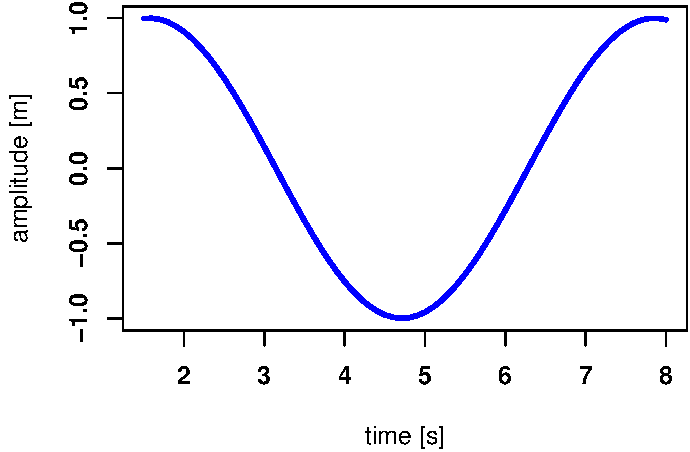
\includegraphics[width=1\linewidth]{paper_files/figure-latex/results-1} \caption{In-text Picture}\label{fig:results}
\end{figure}

Reference to Figure \ref{fig:results}.

\hypertarget{results-and-discussion}{%
\section*{Results and Discussion}\label{results-and-discussion}}
\addcontentsline{toc}{section}{Results and Discussion}

\lipsum[10]

\hypertarget{subsection-2}{%
\subsection*{Subsection}\label{subsection-2}}
\addcontentsline{toc}{subsection}{Subsection}

\lipsum[11]

\hypertarget{subsubsection}{%
\subsubsection*{Subsubsection}\label{subsubsection}}
\addcontentsline{toc}{subsubsection}{Subsubsection}

\lipsum[12]

\hypertarget{subsubsection-1}{%
\subsubsection*{Subsubsection}\label{subsubsection-1}}
\addcontentsline{toc}{subsubsection}{Subsubsection}

\lipsum[14]

\hypertarget{subsection-3}{%
\subsection*{Subsection}\label{subsection-3}}
\addcontentsline{toc}{subsection}{Subsection}

\lipsum[15-20]

\hypertarget{acknowledgments}{%
\section*{Acknowledgments}\label{acknowledgments}}
\addcontentsline{toc}{section}{Acknowledgments}

So long and thanks for all the fish.

\hypertarget{references}{%
\section*{References}\label{references}}
\addcontentsline{toc}{section}{References}

\hypertarget{refs}{}
\leavevmode\hypertarget{ref-Figueredo:2009dg}{}%
Figueredo, Aurelio José, and Pedro S. A. Wolf. 2009. ``Assortative Pairing and Life History Strategy.'' \emph{Human Nature} 20 (3): 317--30. \url{https://doi.org/10.1007/s12110-009-9068-2}.



\end{document}
